%-------------------------
% CV - Yanyu Li
% LaTeX Template (clean, single-column academic CV)
% Compiles with pdflatex or xelatex
%-------------------------

\documentclass[11pt,letterpaper]{article}

% ---------- Packages ----------
\usepackage[utf8]{inputenc}
\usepackage[T1]{fontenc}
\usepackage{lmodern}
\usepackage[margin=0.85in]{geometry}
\usepackage{titlesec}
\usepackage{enumitem}
\usepackage{hyperref}
\usepackage{xcolor}
\usepackage{fancyhdr}
\usepackage{lastpage}
\usepackage{tabularx}
\usepackage{graphicx}
% etaremune removed; using enumerate with [resume] for continuous numbering

% ---------- Colors ----------
\definecolor{linkblue}{HTML}{2B6CB0}
\definecolor{headblue}{HTML}{1A365D}
\definecolor{lightgray}{HTML}{6B7280}

% ---------- Hyperref setup ----------
\hypersetup{
    colorlinks=true,
    linkcolor=linkblue,
    urlcolor=linkblue,
    pdfauthor={Yanyu Li},
    pdftitle={CV - Yanyu Li},
}

% ---------- Section formatting ----------
\titleformat{\section}{
    \vspace{-6pt}\Large\bfseries\color{headblue}\scshape
}{}{0em}{}[\vspace{-6pt}\color{headblue}\titlerule\vspace{-4pt}]

\titleformat{\subsection}{
    \vspace{-2pt}\large\bfseries\color{headblue}
}{}{0em}{}[\vspace{-4pt}]

% ---------- List settings ----------
\setlist[itemize]{leftmargin=*, nosep, topsep=2pt}
\setlist[enumerate]{leftmargin=*, nosep, topsep=2pt}

% ---------- Header / Footer ----------
\pagestyle{fancy}
\fancyhf{}
\renewcommand{\headrulewidth}{0pt}
\fancyfoot[C]{\small\color{lightgray} Yanyu Li \textbar\ Curriculum Vitae \textbar\ Page \thepage\ of \pageref{LastPage}}

% ---------- Custom commands ----------
\newcommand{\cventry}[4]{%
    \noindent\textbf{#1} \hfill \textit{#2} \\
    \textit{#3} \hfill #4 \\[4pt]
}

\newcommand{\pub}[4]{%
    \item #1. \textit{#2}. #3, #4.
}

\newcommand{\pubBold}[5]{%
    \item #1. \textit{#2}. #3, #4. \textbf{#5}
}

% =============================================
\begin{document}

% ---------- Title / Header ----------
\noindent
\begin{minipage}[c]{0.78\textwidth}
    \centering
    {\Huge\bfseries\color{headblue} Yanyu Li} \\[8pt]
    {\large Ph.D., Northeastern University} \\[6pt]
    \href{mailto:li.yanyu@northeastern.edu}{li.yanyu@northeastern.edu} \quad\textbar\quad
    \href{https://scholar.google.com/citations?user=XUj8koUAAAAJ&hl=en}{Google Scholar} \quad\textbar\quad
    \href{https://github.com/liyy201912}{GitHub} \quad\textbar\quad
    \href{https://www.linkedin.com/in/yanyu-li-2216aa17b/}{LinkedIn}
\end{minipage}%
\hfill
\begin{minipage}[c]{0.18\textwidth}
    \raggedleft
    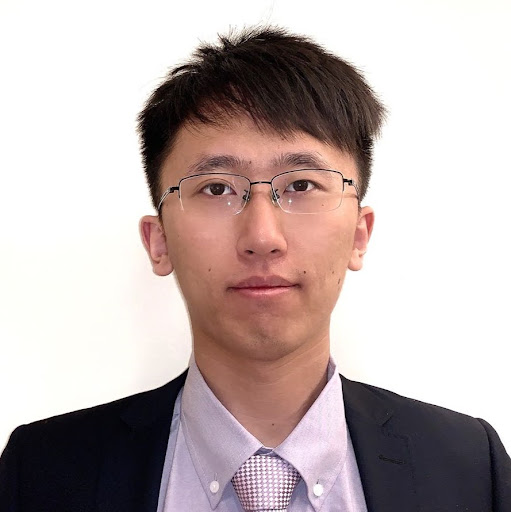
\includegraphics[width=\linewidth,height=2.5cm,keepaspectratio,clip,trim=0 0 0 0]{yanyu.jpg}
\end{minipage}

\vspace{-4pt}

% ---------- Research Interests ----------
\section{Research Interests}

My research focuses primarily on \textbf{Efficient/Mobile Generative AI}: pioneering fast neural networks optimized for edge devices. 
I lead and also hands-on develop the industry-first mobile text-to-image and text-to-video generation projects.
My experience spans over general \textbf{Efficient AI} domains: neural network quantization, pruning, architecture search, and distillation, as well as \textbf{foundational model training}: including web-scale dataset preparation, distributed pretraining across hundreds GPUs, and post-training optimizations. 
I'm now interested in browsing new paradigms for generative AI, and also bringing more appealing applications to real-time (world models, VLMs, MLLMs). 

% ---------- Education ----------
\section{Education}

\cventry{Northeastern University}{Boston, MA}{Ph.D.\ in Computer Engineering}{Sep 2019 -- Aug 2024}
Advisor: Prof.\ Yanzhi Wang

\cventry{Boston University}{Boston, MA}{M.S.\ in Mechanical Engineering (sub-concentration: Robotics)}{Sep 2017 -- Jan 2019}

\cventry{Tsinghua University}{Beijing, China}{B.E.\ in Mechanical Engineering}{Aug 2011 -- Jul 2015}

% ---------- Experience ----------
\section{Experience}

\cventry{Snap Inc.}{Santa Monica, CA}{Research Scientist}{Oct 2024 -- Present}
\begin{itemize}
    \item \textbf{Technical Lead for Industry-First Mobile Video Diffusion:} Spearheaded SnapGen-V---the world's first real-time video diffusion model on mobile devices (5-second video in 5 seconds); architected the full system from DiT compression to on-device deployment, establishing Snap's technical leadership in mobile generative AI.
    \item \textbf{Pioneered Mobile Diffusion Transformer Pipeline:} Led research on efficient DiT architectures (S2DiT, Sprint), novel video autoencoders (H3AE), and streaming video generation; driving next-generation mobile video AI products.
    \item \textbf{Co-led Diffusion Post-Training Research:} Directed cross-functional initiatives in reward fine-tuning, and differentiable reward flow (Diffusion-DRF), advancing image/video quality control at scale.
    \item Mentored junior researchers and interns; projects contributed to CVPR 2025, NeurIPS 2024, and multiple filed patents.
\end{itemize}

\cventry{Northeastern University}{Boston, MA}{Ph.D.\ Research Assistant}{Sep 2019 -- May 2024}
\begin{itemize}
    \item \textbf{Independently led 10+ first-authored projects} resulting in publications at top-tier venues (NeurIPS, CVPR, ICCV, AAAI, IJCAI); dissertation: \textit{Accelerating Large-Scale Generative AI: A Comprehensive Study}.
    \item Spearheaded research on efficient AI spanning neural network quantization, structured pruning, architecture search, and knowledge distillation; applied to CNNs, vision transformers, GANs, and diffusion models.
    \item Collaborated directly with industry partners (Snap Inc., Kuaishou) to bridge academic research and production mobile AI systems.
    \item Served as Teaching Assistant for \textit{EECE 7398: Advances in Deep Learning} and delivered invited guest lecture at NC State University.
\end{itemize}

\cventry{Snap Inc.}{Santa Monica, CA}{Research Intern (Part-time)}{Sep 2022 -- May 2024}
\begin{itemize}
    \item \textbf{Created Industry's First Mobile Image Diffusion Model:} Led SnapFusion from concept to deployment---the first text-to-image diffusion model running on mobile devices under 2 seconds; independently designed architecture compression, step distillation, and latency-quality co-optimization pipeline. Work garnered 290+ citations and established the foundation for Snap's mobile generative AI strategy.
    \item \textbf{Pioneered TextCraftor} for reward-based text-encoder fine-tuning, enabling controllable image quality; commercialized in Snap's consumer products.
    \item Publications at NeurIPS 2023 (SnapFusion) and CVPR 2024 (TextCraftor); 2 US patents filed.
\end{itemize}

\cventry{Snap Inc.}{Santa Monica, CA}{Research Intern (Full-time)}{May 2022 -- Sep 2022}
\begin{itemize}
    \item \textbf{Created EfficientFormer}---first vision transformer achieving true MobileNet-level latency (1\,ms) on mobile hardware with competitive ImageNet accuracy; independently led architecture design, implementation, and ablation studies.
    \item Publications at NeurIPS 2022 and ICCV 2023 (combined 400+ citations); 1 US patent granted; model widely adopted (1,000+ GitHub stars, integrated into timm library).
\end{itemize}

\cventry{CoCoPIE LLC.}{Newton, MA}{Research Intern (Full-time)}{Jun 2021 -- Aug 2021}
\begin{itemize}
    \item Developed compiler-aware algorithm-hardware co-design pipelines for deploying ultra-compressed DNNs on ARM mobile processors, targeting structured pruning patterns compatible with real-time mobile inference.
\end{itemize}

\cventry{Kuaishou Technology US R\&D}{Palo Alto, CA}{Research Intern (Full-time)}{Sep 2020 -- Jan 2021}
\begin{itemize}
    \item Researched GAN compression via structured pruning and dynamic network sparsity, enabling faster video synthesis models; contributed techniques for mobile-deployment-aware model reduction.
\end{itemize}

% ---------- Selected Publications ----------
% Total: 60+ publications | 2,800+ citations | h-index: 24 (as of Feb 2026)

\section{Selected Publications}
\small
\textit{Full list: \href{https://scholar.google.com/citations?user=XUj8koUAAAAJ&hl=en}{Google Scholar} 
\hfill $\dagger$ equal contribution}

\vspace{4pt}
\subsection*{Diffusion Models \& Generative AI (Mobile-First)}

\begin{enumerate}

\pubBold{Y.\ Wu, Z.\ Zhang, \textbf{Y.\ Li}, Y.\ Xu, A.\ Kag, Y.\ Sui, H.\ Coskun, K.\ Ma, A.\ Lebedev, \ldots}
    {SnapGen-V: Generating a Five-Second Video within Five Seconds on a Mobile Device}
    {CVPR}{2025}{(Industry's first mobile video diffusion)}

\pubBold{\textbf{Y.\ Li}, H.\ Wang, Q.\ Jin, J.\ Hu, P.\ Chemerys, Y.\ Fu, Y.\ Wang, S.\ Tulyakov, J.\ Ren}
    {SnapFusion: Text-to-Image Diffusion Model on Mobile Devices within Two Seconds}
    {NeurIPS}{2023}{(Industry's first mobile text-to-image diffusion)}

\pub{J.\ Chen, D.\ Hu, X.\ Huang, H.\ Coskun, A.\ Sahni, A.\ Gupta, A.\ Goyal, D.\ Lahiri, \ldots}
    {SnapGen: Taming High-Resolution Text-to-Image Models for Mobile Devices with Efficient Architectures and Training}
    {CVPR}{2025}

\pub{D.\ Hu, A.\ Gupta, M.\ Gabidolla, A.\ Sahni, H.\ Coskun, \textbf{Y.\ Li}, Y.\ Idelbayev, \ldots}
    {SnapGen++: Unleashing Diffusion Transformers for Efficient High-Fidelity Image Generation on Edge Devices}
    {arXiv preprint}{2026}

\pub{L.\ Zhao, Y.\ Wu, A.\ Lebedev, D.\ Lahiri, M.\ Dong, A.\ Sahni, M.\ Vasilkovsky, \textbf{Y.\ Li}, \ldots}
    {S2DiT: Sandwich Diffusion Transformer for Mobile Streaming Video Generation}
    {arXiv preprint}{2026}

\pub{Y.\ Wu, \textbf{Y.\ Li}, A.\ Kag, I.\ Skorokhodov, W.\ Menapace, K.\ Ma, A.\ Sahni, J.\ Hu, \ldots}
    {Taming Diffusion Transformer for Real-Time Mobile Video Generation}
    {arXiv preprint}{2025}

\end{enumerate}

\subsection*{Diffusion Model Optimization \& Post-Training}

\begin{enumerate}[resume]

\pub{Y.\ Wang, \textbf{Y.\ Li}, S.\ Tulyakov, Y.\ Fu, A.\ Kag}
    {Diffusion-DRF: Differentiable Reward Flow for Video Diffusion Fine-Tuning}
    {arXiv preprint}{2026}

\pub{\textbf{Y.\ Li}, X.\ Liu, A.\ Kag, J.\ Hu, Y.\ Idelbayev, D.\ Sagar, Y.\ Wang, S.\ Tulyakov, J.\ Ren}
    {TextCraftor: Your Text Encoder Can Be Image Quality Controller}
    {CVPR}{2024}

\pub{Y.\ Sui, \textbf{Y.\ Li}, A.\ Kag, Y.\ Idelbayev, J.\ Cao, J.\ Hu, D.\ Sagar, B.\ Yuan, S.\ Tulyakov}
    {BitsFusion: 1.99 Bits Weight Quantization of Diffusion Model}
    {NeurIPS}{2024}

\pub{Z.\ Zhang, \textbf{Y.\ Li}, Y.\ Wu, A.\ Kag, I.\ Skorokhodov, W.\ Menapace, A.\ Siarohin, \ldots}
    {SF-V: Single Forward Video Generation Model}
    {NeurIPS}{2024}

\pub{D.\ Park, M.\ Haji-Ali, \textbf{Y.\ Li}, W.\ Menapace, S.\ Tulyakov, H.J.\ Kim, A.\ Siarohin, \ldots}
    {Sprint: Sparse-Dense Residual Fusion for Efficient Diffusion Transformers}
    {arXiv preprint}{2025}

\pub{X.\ Shen, Z.\ Song, Y.\ Zhou, B.\ Chen, \textbf{Y.\ Li}, Y.\ Gong, K.\ Zhang, H.\ Tan, J.\ Kuen, \ldots}
    {LazyDiT: Lazy Learning for the Acceleration of Diffusion Transformers}
    {AAAI}{2025}

\pub{P.\ Yu, D.\ Luo, T.\ Rupprecht, L.\ Lu, Z.\ Kong, P.\ Zhao, \textbf{Y.\ Li}, O.I.\ Camps, X.\ Lin, \ldots}
    {FasterVD: On Acceleration of Video Diffusion Models}
    {IJCAI}{2024}

\end{enumerate}

\subsection*{Autoencoders \& Generative Architectures}

\begin{enumerate}[resume]

\pub{Y.\ Wu, \textbf{Y.\ Li}, I.\ Skorokhodov, A.\ Kag, W.\ Menapace, S.\ Girish, A.\ Siarohin, \ldots}
    {H3AE: High Compression, High Speed, and High Quality Autoencoder for Video Diffusion Models}
    {arXiv preprint}{2025}

\pub{I.\ Skorokhodov, S.\ Girish, B.\ Hu, W.\ Menapace, \textbf{Y.\ Li}, R.\ Abdal, S.\ Tulyakov}
    {Improving the Diffusability of Autoencoders}
    {arXiv preprint}{2025}

\pub{X.\ Liu, J.\ Ren, A.\ Siarohin, I.\ Skorokhodov, \textbf{Y.\ Li}, D.\ Lin, X.\ Liu, Z.\ Liu, \ldots}
    {HyperHuman: Hyper-Realistic Human Generation with Latent Structural Diffusion}
    {ICLR}{2024}

\pub{Y.\ Gong, Z.\ Zhan, \textbf{Y.\ Li}, Y.\ Idelbayev, A.\ Zharkov, K.\ Aberman, S.\ Tulyakov, \ldots}
    {Efficient Training with Denoised Neural Weights}
    {ECCV}{2024}

\pub{Y.\ Gong$^\dagger$, Z.\ Zhan$^\dagger$, Q.\ Jin, \textbf{Y.\ Li}, Y.\ Idelbayev, X.\ Liu, A.\ Zharkov, K.\ Aberman, \ldots}
    {E$^2$GAN: Efficient Training of Efficient GANs for Image-to-Image Translation}
    {ICML}{2024}

\end{enumerate}

\subsection*{Efficient Vision Transformers}

\begin{enumerate}[resume]

\pubBold{\textbf{Y.\ Li}, J.\ Hu, Y.\ Wen, G.\ Evangelidis, K.\ Salahi, Y.\ Wang, S.\ Tulyakov, J.\ Ren}
    {Rethinking Vision Transformers for MobileNet Size and Speed}
    {ICCV}{2023}{(400+ citations)}

\pub{\textbf{Y.\ Li}, G.\ Yuan, Y.\ Wen, J.\ Hu, G.\ Evangelidis, S.\ Tulyakov, Y.\ Wang, J.\ Ren}
    {EfficientFormer: Vision Transformers at MobileNet Speed}
    {NeurIPS}{2022}

\pub{\textbf{Y.\ Li}, C.\ Yang, P.\ Zhao, G.\ Yuan, W.\ Niu, J.\ Guan, H.\ Tang, M.\ Qin, Q.\ Jin}
    {Towards Real-Time Segmentation on the Edge}
    {AAAI}{2023}

\pub{C.\ Yang, P.\ Zhao, \textbf{Y.\ Li}, W.\ Niu, J.\ Guan, H.\ Tang, M.\ Qin, B.\ Ren, X.\ Lin, \ldots}
    {Pruning Parameterization with Bi-Level Optimization for Efficient Semantic Segmentation on the Edge}
    {CVPR}{2023}

\pub{G.\ Yuan, \textbf{Y.\ Li}, S.\ Li, Z.\ Kong, S.\ Tulyakov, X.\ Tang, Y.\ Wang, J.\ Ren}
    {Layer Freezing \& Data Sieving: Missing Pieces of a Generic Framework for Sparse Training}
    {NeurIPS}{2022}

\pub{\textbf{Y.\ Li}, P.\ Zhao, G.\ Yuan, X.\ Lin, Y.\ Wang, X.\ Chen}
    {Pruning-as-Search: Efficient Neural Architecture Search via Channel Pruning and Structural Reparameterization}
    {IJCAI}{2022}

\end{enumerate}

\subsection*{Hardware-Aware Optimization \& Quantization}

\begin{enumerate}[resume]

\pub{P.\ Dong, J.\ Zhuang, Z.\ Yang, S.\ Ji, \textbf{Y.\ Li}, D.\ Xu, H.\ Huang, J.\ Hu, A.K.\ Jones, \ldots}
    {EQ-ViT: Algorithm-Hardware Co-Design for End-to-End Acceleration of Real-Time Vision Transformer Inference on Versal ACAP}
    {IEEE TCAD}{2024}

\pub{M.\ Jayaweera, \textbf{Y.\ Li}, Y.\ Wang, B.\ Ren, D.\ Kaeli}
    {DEFCON: Deformable Convolutions Leveraging Interval Search and GPU Texture Hardware}
    {IEEE IPDPS}{2024}

\pub{Y.\ Wu, C.\ Wu, G.\ Yuan, \textbf{Y.\ Li}, W.\ Guo, J.\ Rao, X.\ Shen, B.\ Ren, Y.\ Wang}
    {DACO: Pursuing Ultra-Low Power Consumption via DNN-Adaptive CPU-GPU Co-Optimization on Mobile Devices}
    {DATE}{2024}

\pub{G.\ Yang, Y.\ Xie, Z.J.\ Xue, S.E.\ Chang, \textbf{Y.\ Li}, P.\ Dong, J.\ Lei, W.\ Xie, Y.\ Wang}
    {SDA: Low-Bit Stable Diffusion Acceleration on Edge FPGAs}
    {FPL}{2024}

\pub{Z.\ Li, M.\ Sun, A.\ Lu, H.\ Ma, G.\ Yuan, Y.\ Xie, H.\ Tang, \textbf{Y.\ Li}, M.\ Leeser, Z.\ Wang}
    {Auto-ViT-Acc: An FPGA-Aware Automatic Acceleration Framework for Vision Transformer with Mixed-Scheme Quantization}
    {FPL}{2022}

\pub{M.\ Sun, Z.\ Li, A.\ Lu, \textbf{Y.\ Li}, S.E.\ Chang, X.\ Ma, X.\ Lin, Z.\ Fang}
    {FILM-QNN: Efficient FPGA Acceleration of Deep Neural Networks with Intra-Layer, Mixed-Precision Quantization}
    {FPGA}{2022}

\pub{Z.\ Li, G.\ Yuan, W.\ Niu, P.\ Zhao, \textbf{Y.\ Li}, Y.\ Cai, X.\ Shen, Z.\ Zhan, Z.\ Kong, Q.\ Jin}
    {NPAS: A Compiler-Aware Framework of Unified Network Pruning and Architecture Search for Beyond Real-Time Mobile Acceleration}
    {CVPR}{2021}

\pub{\textbf{Y.\ Li}, S.E.\ Chang, M.\ Sun, W.\ Jiang, S.\ Liu, Y.\ Wang, X.\ Lin}
    {RMSMP: A Novel Deep Neural Network Quantization Framework with Row-Wise Mixed Schemes and Multiple Precisions}
    {ICCV}{2021}

\pub{\textbf{Y.\ Li}, S.E.\ Chang,  M.\ Sun, R.\ Shi, H.K.H.\ So, X.\ Qian, Y.\ Wang, X.\ Lin}
    {Mix and Match: A Novel FPGA-Centric Deep Neural Network Quantization Framework}
    {HPCA}{2021}

\end{enumerate}

% ---------- Patents ----------
\section{Patents}

\begin{itemize}
    \item \textit{EfficientFormer Vision Transformer}. US Patent 12,236,668, 2025.
    \item \textit{Text-to-Image Diffusion Model Rearchitecture}. US Patent 12,469,273, 2025.
    \item \textit{Vision Transformer for MobileNet Size and Speed}. US Patent App.\ 18/080,993, 2024.
    \item \textit{Latent Diffusion Model Autodecoders}. US Patent App.\ 18/400,677, 2024.
    \item \textit{Step Distillation for Latent Diffusion Models}. US Patent App.\ 18/434,411, 2024.
    \item \textit{Automatic Image Generation Using Latent Structural Diffusion}. US Patent App.\ 18/429,251, 2025.
    \item \textit{Layer Freezing \& Data Sieving for Sparse Training}. US Patent App.\ 17/893,241, 2024.
\end{itemize}

% ---------- Professional Service ----------
\section{Professional Service}

\noindent\textbf{Conference Reviewer:} NeurIPS, ICCV, ECCV, CVPR, \ldots \\
\textbf{Journal Reviewer:} IEEE TCAD, IEEE TCAS, \ldots

\noindent\textbf{Teaching Assistant (with tech lecturing):} \textit{EECE 7398: Advances in Deep Learning}, Northeastern University, Boston, MA (Fall 2021). Instructor: Prof.\ Yanzhi Wang.

\noindent\textbf{Guest Lecture:} \textit{Real-Time AI and High-Performance Machine Learning}, North Carolina State University (Fall 2022). Instructor: Prof.\ Xipeng Shen.

% ---------- Skills ----------
\section{Technical Keywords}
\textbf{Efficient AI; Transformers; Diffusion Models; PyTorch}; I'm also actively shifting my work style to \textbf{AI coding}. 

% \begin{itemize}
%     \item \textbf{Scientific:} Linear Algebra, Statistics, Supervised/Unsupervised Machine Learning, Convolutional Neural Networks, Transformers, Diffusion Models
%     \item \textbf{Languages \& Frameworks:} Python, PyTorch, TensorFlow, C/C++, CUDA
%     \item \textbf{Tools:} Git, Docker, \LaTeX, Linux
%     \item \textbf{Specialties:} Model compression, neural architecture search, mobile/edge deployment, FPGA acceleration
% \end{itemize}

\vfill

\begin{center}
    \small\color{lightgray}
    Last updated: \today
\end{center}

\end{document}
